\documentclass[a4paper]{article}

\usepackage[T1]{fontenc}
\usepackage[utf8]{inputenc}
\usepackage{graphicx}
\usepackage{fixme}
\usepackage{biblatex}

\usepackage{hyperref}
\addbibresource{biblio.bib}

\newcommand{\eg}{{\textit{e.g.~}}}
\newcommand{\etal}{{\textit{et al.~}}}
\newcommand{\ie}{{\textit{i.e.~}}}

\title{Vers la cognition sociale chez les robots \\ {\large Activités passées et
programme de recherche}}

\author{Séverin Lemaignan}
\date{}

%%% Body
\begin{document}
\maketitle

\section{Activités de recherches passées}
\newrefsection

Ma première contribution dans une conférence internationale remonte à 2006,
lorsque j'étais étudiant en master à l'École Nationale des Arts et Métiers
(ENSAM/ParisTech). Cet article formalisait une ontologie pour décrire les
processsus industriels, et étudiait comment elle pouvait être appliquée à
l'automatisation des lignes de production, via un paradigme
multi-agent~\cite{lemaignan2006mason} (cette publication a été citée depuis
plus de 80 fois).

Depuis cette période, mes activités de recherche se sont focalisées sur cette
question: quels ponts bâtir entre intelligence artificielle (et en particulier,
les techniques de l'ingéneurie des connaissances) et interaction homme-robot.

Je propose de présenter ces travaux en adoptant quatre perspectives
complémentaires : tout d'abord, mon travail sur les outils sémantiques pour la
robotique, ensuite, mes recherches sur le lien entre connaissance et
interaction située, puis mes contributions plus récentes sur le lien entre
cognition robotique et interaction, et enfin, les travaux expérimentaux que
j'ai menés ces dernières années.

Je terminerais cette première partie de mon dossier de candidature en
présentant les autres activités de support scientifique (enseignement,
organisation de colloques et de rencontres scientifiques, développement
logiciels notables).

Toutes les références mentionnées dans cette première partie sont des références
vers des publications dont je suis auteur ou co-auteur.

\subsection{Outils sémantiques pour la robotique%
  \label{semantic-tools-for-robotics}%
}

Paris 5?

ENSAM, MASON
\cite{lemaignan2006mason}, over 80 citations

INRIA, semantic V2V networking, control framework
\cite{mehani2007networking}

\cite{Lemaignan2010} ORO

Talk at INNOROBOT2013

\cite{lemaignan2013explicit}


\subsection{Connaissances et interaction située%
  \label{semantic-tools-for-grounded-interaction}%
}

PhD LAAS/TUM

\cite{ros2010which} (ROMAN best paper award)

\cite{Lemaignan2011} (HRI Pioneers)


\subsubsection{Applications to interaction%
  \label{applications-to-interaction}%
}

Interaction with grounded verbal communication.

\cite{Lemaignan2011a}

\cite{Ros2010a}
\cite{lemaignan2011what}
\cite{lemaignan2011dialogue}
\cite{lemaignan2013talking}

Joint action,...

full paper
The 'CHRIS' suite
\cite{Lallee2010b, Lallee2011, Lallee2012}

workshop
\cite{gharbi2013natural}
\cite{clodic2013on}

\subsection{Cognition pour l'interaction%
  \label{cognition-for-interaction}%
}

Le travail que j'ai mené sur la représentation et la manipulation de la
connaissance pour l'interaction située a naturellement débordé de son périmètre
initial, pour s'éárgir à la question plus générale de la \emph{cognition chez
les robots pour l'interaction}.

Ce champ de recherche est vaste, et est au c\oe ur du projet de recherche que je
présente dans la seconde partie de ce dossier.

J'ai travaillé sur cette question sous deux angles : une perspective
intégrative, d'une part, et une perspective exploratoire \fxnote{...quel mot}.

J'ai ainsi coordonné l'écriture de plusieurs articles de journaux
\cite{alami2011when, Lemaignan2012, lemaignan2014human} qui présentent comment
la manipulation explicite de connaissances symboliques ouvre des voies nouvelles
pour l'intégration des multiples processus décisionels au sein d'une
architecture robotique complexe.

Dans~\cite{lemaignan2014human} en particulier, je présente en particulier les
principaux défis que l'interaction homme-robot pose à l'intelligence
artificielle, en termes de \emph{grounding}, de modèles mentaux, d'attention et
d'action conjointe, d'interaction naturelle multi-modale ou encore d'analyse
spatiale, temporelle et contextualisée de situation. Je montre aussi que ces
questions peuvent être en partie abordées de manière commune en définissant les
interfaces entre modules décisionels en terme de sémantique échangée.

Parallèlement à cet effort de synthèse au niveau de l'architecture globale du
robot, j'ai mené plusieurs expériences centrées sur des aspects cognitifs
précis. Ainsi, les expériences de \emph{False Beliefs}~\cite{Warnier2012a},
étroitement liées à la mise en place d'une théorie de l'esprit chez le robot.

Ainsi aussi, le travail que j'ai mené durant mon post-doctorat au LAAS-CNRS
(2012-2013) sur les besoins spécifiques de représentations pour l'interaction.
L'objectif était de concevoir une technique de représentation fusionnant le
\emph{Umwelt} (\emph{monde propre}) spatial et temporel du robot en un modèle
amodal pouvant servir de point d'entrée pour les fonctions cognitives
supérieures du robot.

Le prototype que j'ai developpé est construit autour de l'idée de \emph{mondes}
que le robot peut manipuler en fonction de son contexte et de ses besoins.
Chaque monde consiste en une représentation géométrique et une histoire dans
lequel on peut librement naviguer. Les différents mondes peuvent se synchroniser
entre eux, mais aussi évoluer independament (on peut alors les concevoir comme
des mondes hypothétiques, adaptés par exemple pour simuler et représenter le
résultat d'une planification).

Par ailleurs, je me suis aussi intéressé à la question de la cognition pour
l'interaction sous l'angle complémentaire des mécanismes cognitifs
\emph{humains} en jeu durant une interaction.

J'ai commencé à m'interesser à cet aspect dans le cadre de la robotique
pédagogique. D'abord de manière expérimentale au sein de l'association Planète
Sciences~\cite{stinckwich2007squeakbot}, puis de manière plus théorique en
suivant un Master Recherche à l'Université Paris 5 dans le domaine des
Environments Informatiques pour l'Apprentissage Humain (EIAH), ce qui n'a permis
d'acquérir un certain nombre de bases en Human-Computer Interaction (HCI), en
particulier en ergonomie.

Ces deux premières expériences ont facilité choix de mon post-doctorat à l'École
POlytechnique Fédérale de Lausanne, où j'ai pris en charge la coordination des
activités robotiques au sein du laboratoire d'ergonomie éducative. Ce
laboratoire (CHILI-EPFL) est connu pour son expertise dans l'étude des
interactions homme-machine et homme-homme durant les phases d'apprentissage. J'y
ai acquis le savoir-faire nécessaire à la menée et l'analyse d'expériences
in-situ (écologiquement valides) et controllées.

Je supervise deux projets principaux. Le premier s'intéresse aux interactions
sur la durée entre le robot Ranger et des enfants~\cite{fink2014which}. Il m'a
permis, entre autres, d'étudier l'impact des comportements anthropomorphiques
sur l'interaction homme-robot sur le long terme~\cite{lemaignan2014dynamics}. Il
apparait en particulier que les mécanismes cognitifs en jeu chez l'homme lors
d'une interaction suivie dans le temps ont été peu étudié, alors qu'ils sont
critiques pour concevoir et adapter le comportement du robot sur le long terme.

Le second projet repose sur l'idée du \emph{learning by teaching}, et propose de
mettre en place une interaction enfant-robot durant laquelle l'enfant
\emph{montre} au robot (un Nao) comment écrire. La question que l'on se pose est
de savoir si une telle situation peut créer une forme interaction originale qui
permette d'établir une relation pérenne et qui soutienne efficacement
l'apprentissage.

\subsection{Mener des expériences en HRI}

Table \ref{experiences} lists the main experiments I have conducted over the
last 4 years.

\begin{table*}
\begin{center}

    \begin{tabular}{lp{5.5cm}l}
\bf{Expérience} & Objet principal & Référence \\
\hline
{\it Point \& Learn} (2010) & Acquisition interactive de connaissances & \cite{Lemaignan2010} \\
{\it Spy Game} (2010) & Discrimination interactive d'objets & \cite{ros2010which} \\
{\it Moving to London} (2011) & Interaction multi-modale, \newline prise de perspective & \cite{lemaignan2011what} \\
{\it Roboscopie} (2011) & Théâtre, \newline réflexion sur le futur de la HRI & \cite{lemaignan2012roboscopie} \\
{\it Cleaning the table} (2011) & Intégration complète & \cite{alami2011when} \\
{\it I'm in your shoes} (2012) & Fausses croyances & \cite{Warnier2012a} \\
{\it Give me this} (2012) & Manipulation naturelle conjointe & \cite{gharbi2013natural} \\
{\it Aperitif time} (2012) & Interaction multi-modale, \newline prise de perspective & \cite{lemaignan2013talking} \\
{\it CoWriter 1} (2013) & \emph{Expérience enfant-enfant}, \newline protocoles
d'interaction, expérience de terrain &  \\
{\it Ranger} (2013) & Expérience enfant-robot, \newline projections cognitives en HRI &
\cite{fink2014which, lemaignan2014dynamics} \\
\hline

\end{tabular}
\end{center}
\caption{Principales expériences menées en interaction homme-robot.}
\label{experiences}
\end{table*}

postdoc EPFL

\cite{fink2014which}


\subsection{Autres activités de support scientifique}

Dans cette dernière section, je propose de parcourir brièvement mes autres
activités scientiques, afin d'inscrire ma candidature dans le cadre plus large
de l'animation de la vie scientifique.

\subsubsection{Enseignement et encadrement}

Depuis mon entrée dans la recherche à l'INRIA en 2006, j'ai souhaité développer une
activité d'enseignement en parallèle de mon travail de recherche.

J'ai été ainsi assistant d'enseignement en mécatronique à Mines ParisTech
pendant un an (sous la supervision de Bruno Steux), puis durant mon doctorat,
j'ai été moniteur à l'INSA Toulouse, impliqué en particulier sur les travaux
dirigés et pratiques en Prolog, sur les ontologies, en Java, ADA et SQL.

J'ai aussi organisé et animé de nombreux ateliers et tutoriels dans plusieurs
domaines de la robotique et du développement logiciel, et souvent destinés aux
jeunes chercheurs. Je suis ainsi intervenu sur la programmation avec ROS, les
techniques de développement collaboratif (comme GIT), les cycles de
développement, l'utilisation d'outils sémantiques comme les ontologies. J'ai
organisé plusieurs tutoriels internationaux sur la simulation en robotique (en
particulier, lors de la conférence EURON2012 au Danemark), et je suis, depuis
2005, formateur au sein de l'association française \emph{Planète Sciences} sur
les questions de robotique pédagogique.

Par ailleurs, j'ai été amené à encadrer plusieurs étudiants ces dernières
années. Une dizaine d'étudiants de master au total (dont le travail, pour
certains, a débouché ensuite sur des publications, comme~\cite{Lemaignan2011a}),
et, durant mon post-doctorat à l'EPFL, deux doctorants (Julia Fink et Shruti
Chandra). L'une travaille sur la question de l'interaction homme-machine sur le
long terme, avec en particulier une évaluation des effets de
l'anthropomorphisme, l'autre travaille sur l'utilisation de robots compagnons
pour soutenir les enfants en difficulté face à l'apprentissage de l'écriture.

\subsubsection{Associations scientifiques et dissémination}

Outre mon implication, déjà mentionnée, dans l'association de diffusion de la
culture scientifique \emph{Planète
Sciences}, dont j'ai présidé pendant deux ans la section robotique, j'ai été,
durant mon doctorat, vice-président de l'association \emph{InCOGnu}, antenne
Sud-Ouest de la Fédération Française des Étudiants et Jeunes Chercheurs en
Sciences de la Cognition (FRESCO). Mon activité au sein de cette association de
jeunes chercheurs m'a permis de m'ouvrir assez largement aux divers aspects de
la recherche en sciences cognitives, en particulier à travers les conférences
mensuelles que nous avons proposés, et où intervenait des chercheurs confirmés.
C'est aussi dans le cadre d'InCOGnu que j'ai participé à l'organisation de la
conférence CJCSC (Colloque des Jeunes Chercheurs en Sciences Cognitives) à
Toulouse en 2009.

Plus récemment, j'ai organisé et animé en 2012 le premier workshop international
sur le simulateur MORSE auquel une quinzaine de chercheurs de quatre pays ont
participé.

Je suis par ailleurs relecteur régulier pour les principales conférences en
robotique (IROS, ICRA, RoMAN, HRI).

Parmis les actions que j'ai mené à destination du grand public, la pièce de
théâtre Roboscopie (qui a débouché sur une
publication,~\cite{lemaignan2012roboscopie}) peut être mentionné : à l'automne
2011, j'ai mis en place, en collaboration avec un metteur en scène et un
comédien professionel, une pièce de théâtre d'une vingtaine de minutes dans
laquelle un robot PR2 donne la réplique à un homme. La pièce interroge sur un
mode métaphorique comment hommes et robots peuvent trouver un espace de vie et
de compréhension mutuel. La pièce a été présentée à environ 400 personnes durant
le festival Novela.

\subsubsection{Contributions logicielles notables}

Au-delà des développements logiciels directement en lien avec mon travail de
doctorat, et précédemment mentionnés (ORO~\cite{Lemaignan2010}, {\sc
Dialogs}~\cite{Lemaignan2011a}), je me suis impliqué dans le développement de
plusieurs autres projets dont la portée est significative dans la communauté
robotique.

Le premier de ces projets est le simulateur MORSE~\cite{Echeverria2011,
echeverria2012simulating}. Le projet a pris une ampleur certaine, avec plus de
25 contributeurs du monde entier, son intégration officielle dans le projet
Debian, et un workshop annuel.

J'en suis le concepteur initial, l'un des principaux contributeurs, et le
principal animateur de la communauté des développeurs. J'ai en particulier
travaillé sur l'utilisation de MORSE pour simuler des interactions
homme-robot~\cite{lemaignan2012morse}.

ROS (Robot Operating System) est un autre projet dans lequel je suis impliqué.
J'ai plusieurs contributions dans le noyau de ROS et je me suis aussi fortement
impliqué dans l'adaptation de ROS au robot Nao, en particulier pour faciliter
l'installation de ROS sur ce robot.

Je suis aussi impliqué dans la conception d'outils logiciels plus spécialisés,
comme GenoM~\cite{mallet2010genom3}.

\subsection{Pour conclure}

Pour conclure cette première partie, je souhaiterais souligner deux traits de
mon parcours : sa dimension internationale, et l'importance de
l'interdisciplinarité.

Mon parcours de recherche démarre à la période du master : j'ai fait le choix de
suivre un cursus d'ingénieur franco-allemand, qui m'a conduit près de deux ans
en Allemagne, au Karlsruhe Institute of Technology (KIT), et m'a finalement
permis d'obtenir en 2006 la médaille d'or de l'ENSAM/ParisTech. J'ai aussi,
pendant ce master, mené pendant six mois des travaux de recherche en physique
fondamentale au Paul Scherrer Institute en Suisse, ce qui a représenté ma
première immersion dans le monde académique à proprement parler.

Suite à cela, et bien que cela ne fasse pas partie de mon parcours de chercheur,
j'ai voyagé pendant une année autour du monde (2007-2008), expérience
importante tant au niveau personnel qu'au regard de mon ouverture à
l'international.

Ensuite, j'ai souhaité organisé mon doctorat en co-tutelle à son tour, cette
fois avec la Technische Universität de Munich (TUM), ce qui m'a conduit à
nouveau à séjourner plusieurs mois en Allemagne. Mon doctorat allemand, noté, a
reçu la meilleure note possible (\emph{Cum Suma Laude}).

Enfin, le post-doctorat que je réalise actuellement à l'École Polytechnique
Fédérale de Lausanne (EPFL) est la plus récente escale internationale de mon
parcours.

Cet itinéraire international reflète la diversité des environnements
intellectuels dans lesquels j'ai évolué, et m'a permis mieux appréhender le
tissu scientifique européen, en particulier dans le domaine de la robotique
cognitive.

Le deuxième aspect particulier de mon parcours est sa dimension
interdisciplinaire : depuis la période du master, durant laquelle j'ai suivi en
parallèle une formation d'ingénieur et un master dans le domaine de
l'intelligence artificielle appliquée à l'éducation, j'ai tenté de garder une
ouverture sur les questions d'éducation, et plus largement, de cognition
humaine. C'est ainsi que je me suis impliqué dans l'association des jeunes
chercheurs en sciences cognitives, c'est ainsi aussi que j'ai choisi de
rejoindre en post-doctorat un laboratoire centré sur les technologies pour
l'éducation, avec un savoir-faire fort dans le domaine de l'expérimentation
homme-machine. J'y ai acquis une expérience essentielle pour pouvoir aujourd'hui
mener des expériences en HRI qui soient pertinentes, écologiquement valides, et
méthodologiquement solides.

\printbibliography


%%%%%%%%%%%%%%%%%%%%%%%%%%%%%%%%%%%%%%%%%%%%%%%%%%%%%%%%%%%%%%%%%%%%%%%%%%%%%%%%%%%%%%%%%%%%%%%%%%%%%%%
%%%%%%%%%%%%%%%%%%%%%%%%%%%%%%%%%%%%%%%%%%%%%%%%%%%%%%%%%%%%%%%%%%%%%%%%%%%%%%%%%%%%%%%%%%%%%%%%%%%%%%%
%%%%%%%%%%%%%%%%%%%%%%%%%%%%%%%%%%%%%%%%%%%%%%%%%%%%%%%%%%%%%%%%%%%%%%%%%%%%%%%%%%%%%%%%%%%%%%%%%%%%%%%

\section{Projet de programme de recherche}
\newrefsection

La présentation de mes activités de recherche passées peut être comprise comme
plusieurs regards sur la question de la cognition sociale chez les robots : la
question de la représentation et de la manipulation des connaissances en premier
lieu, la question des pré-supposés à l'interaction naturelle (et verbale en
particulier) ensuite, la question de la cohérence et de la faisabilité d'une
architecture cognitive intégrée, la question de l'évaluation de l'engagement
homme-robot sur le long terme...

Ces différentes facettes sont autant de pièces d'un puzzle auquel je propose de
travailler directement : \textbf{comment comprendre l'idée de \emph{cognition
sociale} chez le robot, comment la construire, comment l'évaluer ?}

Ce projet articule plusieurs axes, que j'expose plus en détails ci-après. La
première question que l'on peut poser est : Que nous enseignent les sciences
cognitives \emph{humaines} en terme de compétences cognitives nécessaires à
l'interaction entre agents, et en terme d'évaluation de ces compétences ? Une
synthèse des travaux existants en sciences humaines, et le travail d'adaptation
à la robotique sont des manques bien identifiés pour avancer sur les questions
d'interaction sociale entre hommes et robots.

La question de recherche fondamentale que cela ouvre est le travail de
compréhension, de définition et d'application de l'idée de cognition sociale en
robotique. Il s'agit ici d'articuler une problématique aujourd'hui floue car
complexe, en re-pensant l'existant ((neuro-)sciences cognitives, donc, mais
aussi architectures cognitives telle qu'on les connait en intelligence
artificielle) dans le cadre de la robotique sociale, avec ses dimensions
particulières (relations interpersonnelles, incarnation, sous-spécification,
dynamique). Il s'agit non seulement de construire l'idée de cognition sociale
chez le robot, mais aussi de l'envisager de manière concrête, en terme
d'implémentation sur des robots.

Un aspect opérationel qui en découle, et dont je propose de faire un de mes axes
de recherche, est la question de la \emph{représentation} de l'environement
spatial, temporel, social et contextuel du robot. La litérature s'intéresse
essentiellement aux deux premiers points. Il me semble que les deux derniers
sont des objets encore peu étudiés et pourtant essentiels pour une prise de
décision autonome et complexe pour l'interaction homme-robot.

Enfin, je souhaite inscrire ce programme de recherche dans une perspective
expérimentale forte. La menée systématique d'expériences d'interaction en milieux
écologiquement valides reste rare et sujette à des faiblesses méthodologiques.
En m'appuyant sur l'expérience que j'ai acquise dans ce domaine, je pense
travailler à la mise en place d'un référentiel expérimental dont la méthodologie
est solide, et sur lequel je pourrais m'appuyer pour valider la réflexion sur la
cognition sociale chez le robot.

\subsection{Vers la cognition sociale chez le robot}

Comme je l'ai présenté dans~\cite{lemaignan2014human}, si la robotique cognitive
, qui hérite de la psychologie cognitive, s'intéresse aux processus mentaux
comme l'\emph{attention}, l'utilisation du \emph{langage}, la \emph{mémoire} ou
les processus de \emph{prise de décision}, la cognition sociale y ajoute les
aspects lié à la prise en compte des interactions avec d'autres agents :
\emph{représentation des croyances}, \emph{prise de perspective}, \emph{action
conjointe}, et tous les aspects liés à la \emph{communication}.

L'idée de \emph{robotique cognitive} n'est pas récente (elle est mentionnée dès
le début des années 1990 par Reiter~\cite{Levesque2008}), et est déjà établie
comme un champ de recherche actif, formant le pendant des approches
développementales de la robotique. Si ce domaine est ancien, il est cependant
traité de manière essentiellement atomique en robotique : les compétences
cognitives sont implémentées et testées indépendement les unes des autres, et
comme le note Kurup~\cite{kurup2012what}, ce n'est que récemment que la
robotique s'intéresse aux architectures cognitives holistiques développées en
intelligence artificielle. Les travaux de Trafton~\etal sur
ACT-R/E~\cite{trafton2013act} ou les recherches menées par Baxter dans le cadre
du projet européen ALIZ-E~\cite{baxter2013cognitive} en sont des exemples
récents.

ACT-R/E est un exemple intéressant dans la mesure où l'architecture est conçue
en premier lieu pour l'interaction homme-robot, et elle est évaluée en se
référant explicitement à la psychologie dévelopmentale. Elle illustre aussi le
chemin qui reste à parcourir dans ce domaine : bien qu'étant une architecture
cognitive globale, elle n'a été testée que sur des compétences cognitives
isolées, en laboratoire, et ignore largement les problématiques d'ancrage
symbolique (le robot raisonne sur un environnement simplifié, et les modalités
de communication sont elles aussi simples -- pas d'interaction linguistique, par
exemple).


\paragraph{Métriques de la cognition en robotique}

L'une des difficultés importantes à laquelle la communauté de la robotique
cognitive fait face est l'absence de référentiel permettant d'évaluer (et donc
de comparer et mesurer les progrès) les capacités cognitives de nos robots.
Cela tient à deux raisons principales : d'une part, comme nous venons de le
voir, le périmètre de ce qu'on appelle la robotique cognitive est relativement
mal défini, ce qui rend difficile la création d'une mesure globale des capacités
cognitives ; d'autre part la plupart des outils d'évaluation à notre disposition
viennent de l'étude de la cognition humaine, et sont concrètrement souvent
difficile à appliquer aux robots car la ``hiérarchie'' des compétences
cognitives chez les robots est très différente de ce que l'on rencontre chez
l'homme : les compétences langagières, pour prendre exemple symbolique, sont
difficilement comparable. La production verbale est considérée pour un robot
comme un problème moins difficile (essentiellement traitée par la synthèse
vocale) que la compréhension orale (qui requiert, outre la reconnaissance
vocale, une analyse syntaxique et sémantique). Or les tests de langage que l'on
rencontre en psychologie cognitive vont typiquement tester la capacité à parler
en assumant que l'enfant peut comprendre ce qu'on lui dit.

De fait, la communauté robotique s'appuie aujourd'hui essentiellement sur des
évaluations qualitatives. Langley~\etal\cite{Langley2006} suggère ainsi cinq
dimensions d'évaluation : la \emph{généralité} du système (peut-il s'adapter à
une nouvelle tâche?), la \emph{rationalité} ou pertinence des
inférences/raisonnements/décisions que le système prend, la \emph{réactivité} et
la \emph{persistance} qui évalue si le comportement du système est approprié en
cas de changements non-anticipés, la capacité du système à \emph{ameliorer sa
performance} comme fonction des connaissances supplémentaires qu'on lui fournit,
et enfin, \emph{l'autonomie} du système. On le voit, ces dimensions sont
générales, et peu opérationelles.

Un certain nombre d'outils issus de la psychologie cognitive ont déjà été
explorés de manière concrête sur des robots, comme les expériences d'inversion
de rôle~\cite{Lallee2010b}, de croyances fausses (\emph{False
Beliefs}~\cite{Leslie2000}), lié à la théorie de l'esprit~\cite{Breazeal2006,
Warnier2012a, trafton2013act}, ou encore le \emph{Token
test}~\cite{DiSimoni1978} pour l'évaluation de certaines compétences
linguistiques~\cite{Mavridis2006}. Ces expériences ont montré qu'il était
possible et utile de ré-utiliser en les adaptant des tests de psychologie
cognitive en robotique. Elles restent cependant ponctuelles, et une travail plus
systématique et plus global reste à faire. D'autant plus que, comme l'ont
récemment souligné Zhang~\etal\cite{zhang2013evaluation}, les environements et
métriques existants pour l'évaluation des performances cognitives des robots se
focalisent pour la plupart sur des capacités physiques, et ne requièrent pas de
capacités avancées de représentation et manipulation de connaissance.

Eux-même proposent leur une métrique basée sur la mesure du \emph{Fitness to
Ideal Model} (FIM) d'un comportement, qu'ils corrèlent à la \emph{longueur de
description} (DLen) de la commande qui a déclenchée le comportement. L'hypothèse
étant que, pour un comportement donné, plus le robot a des capacités cognitives
avancées, plus courte (c'est à dire, sous-spécifiée) pourra être la commande, le
robot inférant le reste. Cette piste est intéressante, et est à mettre en
relation avec d'autres approches issues des sciences cognitives humaines.

Mon objectif est ici de rechercher et de construire un référentiel solide et
opérationnel pour l'évaluation des compétences cognitives des robots, en
s'intéressant à la fois à l'évaluation de chaque capacité cognitive
indépendente, et à la fois à des métriques globales de l'activité cognitive du
robot. Dans~\cite{lemaignan2013explicit}, je propose une piste à explorer à ce
sujet en définissant la notion de \emph{charge cognitive} du roboten terme de
flux de connaissances à l'intérieur de l'architecture logicielle du robot.

Plus généralement, ce premier axe de recherche que je propose s'inscrit dans la
perspective des architectures cognitives pour la robotique sociale. Il s'agit de
réaliser d'abord la synthèse des travaux en sciences cognitives aussi bien en
terme de construction de l'interaction que d'évaluation des compétences
cognitives, puis ensuite l'alignement de ces résultats avec les spécificités de
la robotique. Les objectifs sont d'une part la définition du périmètre de la
cognition sociale en robotique, d'autre part la création d'un référentiel
d'évaluation des compétences cognitives des robots d'interaction.


\subsection{La représentation du monde comme fondation de la cognition}

\begin{figure}
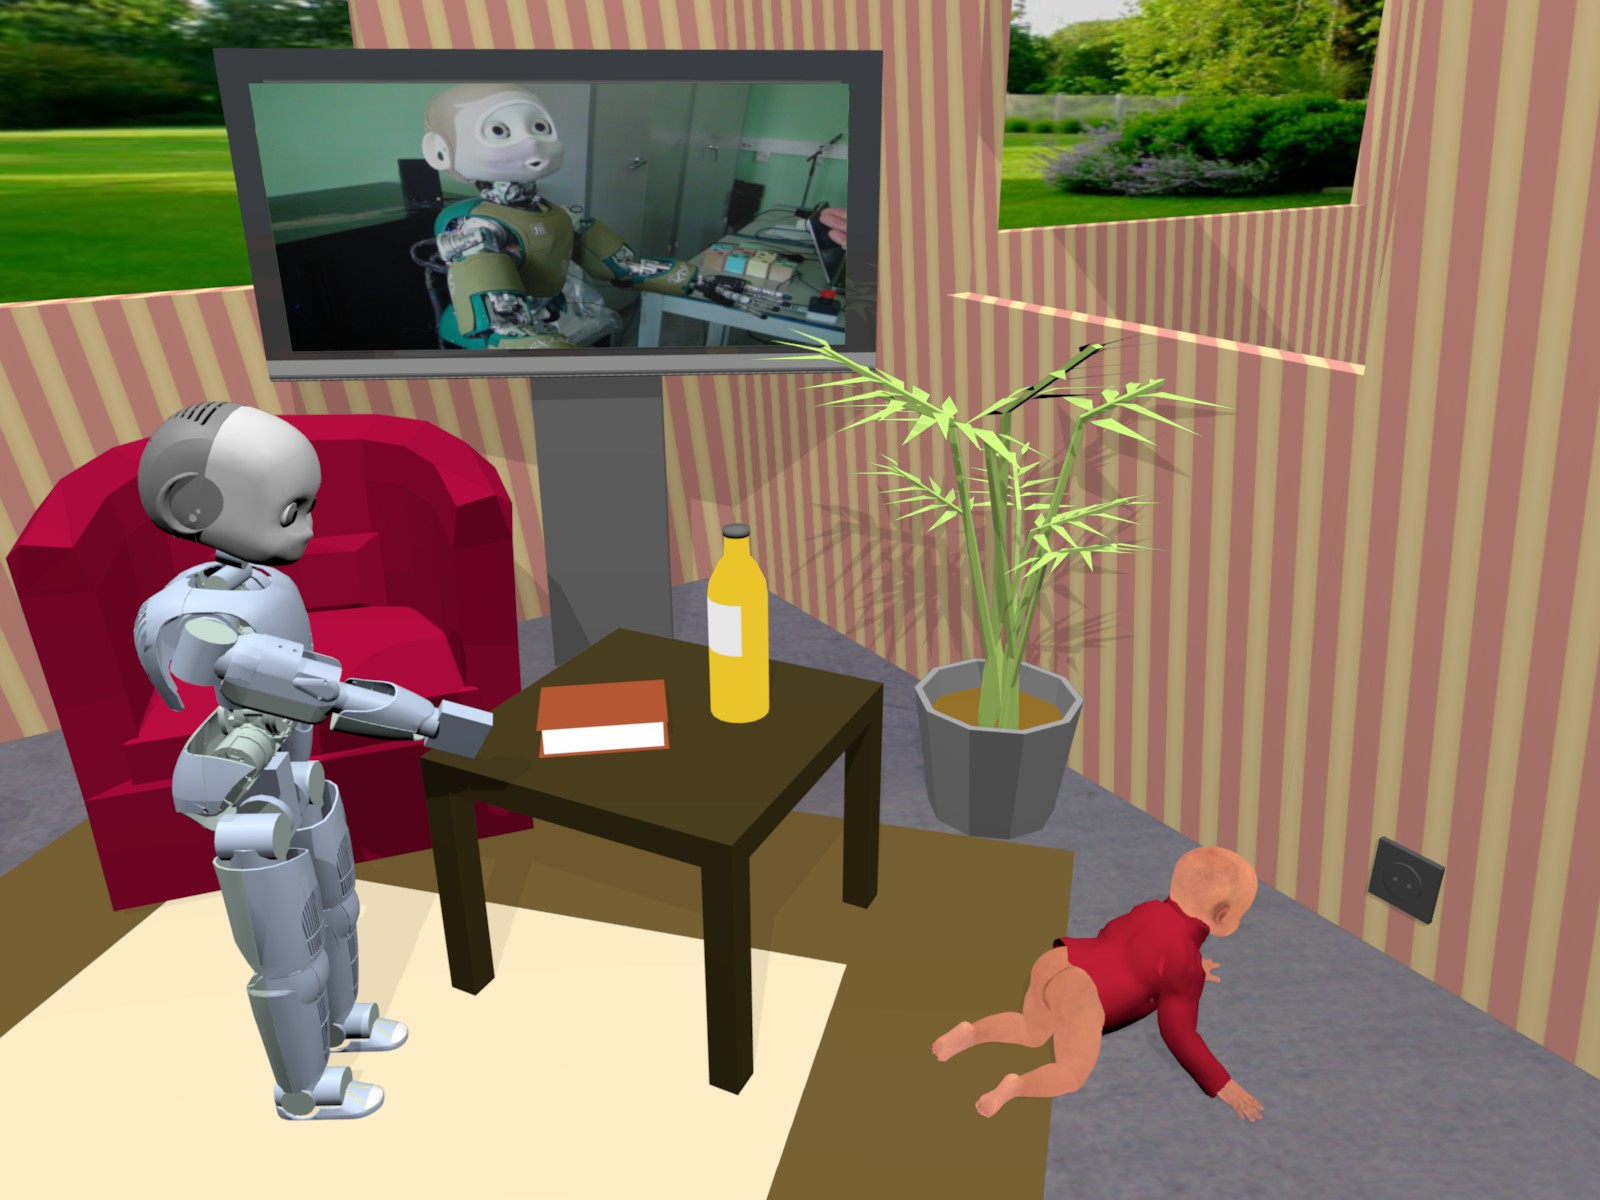
\includegraphics[width=\textwidth]{figs/robots_home_baby_socket.jpg}
\label{babyplug}
\end{figure}

\subsection{Un programme expérimental ambitieux}

Je propose de matérialiser les axes de recherche que j'ai présenté autour de
quatre objectifs expérimentaux, qui vont de la conception et de
l'implémentation d'une méthodologie expérimentale pour évaluer les compétences
cognitives des robots, au déploiement d'un robot manipulateur mobile de type
PR2 dans une famille non-experte pour une durée longue (supérieure à un mois).

Le premier objectif consiste donc à formaliser une méthodologie expérimentale
pour l'évaluation des capacités cognitives d'un robot. Cette méthodologie doit
être reproductible sur différentes plateformes robotiques. Je me fixe un horizon
à J+12 mois pour atteindre cet objectif, qui pré-suppose un travail d'analyse et de
synthèse des outils existants en psychologie dévelopmentale et cognitive, ainsi
qu'en intelligence artificielle.

La seconde expérience vise à démontrer l'intérêt d'une représentation unifiée de
l'environnement du robot: on se place dans plusieurs scénarios d'interaction
dans l'esprit de la figure~\ref{babyplug}, pour lesquels une interprétation
correcte nécessite de combiner représentations géométriques et symboliques,
d'être capable de représenter des états futurs hypothétiques, et de reconnaitre
et mobiliser un ensemble de contextes complémentaires. On évalue alors la
qualité et la pertinence du modèle et de l'interprétation de la scène créé par
le robot, en les comparant aux interprétations produites par un humain. La mise
en place de cette expérience requiert des développements logiciels conséquents,
et je me fixe un horizon à environ J+18 mois.

La troisième expérience s'intéresse aux facteurs cognitifs d'une interaction
longue. L'objectif est de déployer des robots type Nao avec des schémas
d'interaction simples (tâches du type aide à la cuisine avec les recettes ou
lecture d'histoire pour les enfants) dans des familles sur des périodes longues
(de l'ordre de 3 mois) afin d'analyser quels sont les facteurs, tant humains que
robotiques, qui permettent d'établir un engagement durable. Pour cette
expérience, je souhaite d'échelonner plusieurs déploiements dans plusieurs
familles en parallèle, et cette expérience pourrait s'étaler de J+20 mois à J+26
mois.

Enfin, en s'appuyant sur les enseignements issus de l'expérience précédente, le
dernier objectif expérimental, plus ambitieux, consiste à déployer un robot
complexe type PR2, dans une famille, pour une durée longue, et avec un
répertoire d'interactions étendu, incluant autonomie complète, dialogue
multi-modal, manipulation conjointe. Je situe cet objectif expérimental à un
horizon d'environ J+30 mois.

Ce programme expérimental ambitieux mais que j'estime réaliste, vise à faire
avancer significativement l'état de l'art en ce qui concerne la robotique
d'interaction. La plateforme expérimentale proposée par l'ISIR est l'une des rares
en France qui permette d'envisager raisonnablement ce programme, et c'est aussi
une des raisons principales pour lesquelles je souhaite rejoindre ce
laboratoire.

\subsection{Pour conclure}

\printbibliography

\end{document}
